\documentclass{article}
\usepackage[utf8]{inputenc}

\title{MATH3160 — Portfolio 2.2-3.3}
\author{Mike Medved}
\date{September 11th, 2022}

\usepackage{color}
\usepackage{amsthm}
\usepackage{amssymb} 
\usepackage{amsmath}
\usepackage[margin=1in]{geometry} 
\usepackage{listings}
\usepackage[dvipsnames]{xcolor}
\usepackage{tikz}

\begin{document}

\maketitle

\section{Deliverables}

\subsection{Properties of Probability}

\begin{itemize}
    \item The probability of an Impossible Event must be zero.
    \begin{itemize}
        \item Let $A \subseteq S, P(A) = P(A \cup \emptyset) \Rightarrow P(A) = P(A) + P(\emptyset) \Rightarrow P(\emptyset) = 0$
    \end{itemize}
    \item The probability of a Contrary Event, $P(A^c)$ is one minus the probability of $P(A)$.
    \begin{itemize}
        \item Let $A$ be an event, $P(A^c) = 1 - P(A)$
    \end{itemize}
    \item If $A$ is contained within $B$, then $P(A) \leq P(B)$.
    \begin{itemize}
        \item Let $A \subseteq B$, then $P(B) = P(A) + P(B - A) \Rightarrow P(B) - P(A) = P(B - A) \geq 0$
    \end{itemize}
\end{itemize}

\subsection{Famous Problems}

\begin{enumerate}
    \item Strange Dice
    \begin{enumerate}
        \item The interesting idea behind the strange dice problem is that given a set of three dice, where each die is a three-faced die with three distinct values, we can show that the probability of Die A beating Die B is $55\%$, and the probability of Die B beating Die C is also $55\%$. You would think that the probability of Die A beating Die C would be higher than $55\%$, but it is actually $44.4\%$.
        
        $\hfill \break$
        This is significant because Player 2 has a substantial advantage over Player 1, since Player 1 merely chooses a die from the three, but Player 2 can mathematically determine which die to choose in order to beat Player 1. 
    \end{enumerate}
    \item Chevalier de Mere
    \begin{enumerate}
        \item The interesting idea behind the Chevalier de Mere problem is that given a fair die, the probability of rolling a single six in six rolls is approximately 0.5177, however rolling a double six on two dies in 24-rolls is always slightly lower, approximately 0.4914. This is significant because it shows that the probability of rolling a double six is lower than the probability of rolling a single six, which is a bit counter-intuitive.
    \end{enumerate}
    \item Birthday Paradox
    \begin{enumerate}
        \item The interesting idea behind the Birthday Paradox problem is that given a group of $n$ people, the probability that two people share the same birthday is approximately $1 - \frac{365!}{(365-n)!365^n}$. This is significant because it shows that the probability of two people sharing the same birthday is not zero, and is actually quite high.
        
        $\hfill \break$
        The reason why the probability is actually quite high is because when we compute the contrary event $A^c$, we must take $A=1-A^c$, and since the denominator of $A^c$ grows exponentially with respect to $n$, when we subtract this value from 1, we get a high percentage.
    \end{enumerate}
\end{enumerate}

\subsection{Conditional Probability}

The Conditional Probability of an event refers to the probability of an event occurring given that another event has already occurred, this may or may not influence the final probability, as some events are independent of one-another.

$\hfill \break$
\textbf{Definition:} Let $S$ be a sample space, $P$ be a probability resting within the sample space, and events $A, B \in S$ such that $P(B) > 0$. The conditional probability $P(A|B)$ can be represented by the formula:

$$
    P(A|B) = \frac{P(A \cap B)}{P(B)}
$$

$\hfill \break$
Now that we know what the definition of conditional probability is, we can take a closer look at some of it's properties.

$\hfill \break$
\textbf{Properties:}

\begin{enumerate}
    \item Product Rule (2 Sets)
    \begin{enumerate}
        \item The product rule for two sets states that given $P(A \cap B)$, you can rewrite it as $P(A)*P(B|A)$.
    \end{enumerate}

    \item Product Rule (3 sets)
    \begin{enumerate}
        \item The product rule for three sets is similar, but instead of $P(A \cap B)$, we have $P(A \cap B \cap C)$, and as such, we can rewrite it as $P(A)*P(B|A)*P(C|A \cap B)$.
    \end{enumerate}
    
    \item Generalized Product Rule
    \begin{enumerate}
        \item The generalization of the two above rules goes as follows: Given $n$ sets, $P(A_1 \cap A_2 ... A_{n-1} \cap A_n)$ can be rewritten as $P(A_1)*P(A_2|A_1)*P(A_3|A_1 \cap A_2)*...*P(A_{n-1}|A_1 \cap A_2 ... A_{n-2})*P(A_n|A_1 \cap A_2 ... A_{n-1})$.
    \end{enumerate}
    
    \item Law of Total Probability
    \begin{enumerate}
        \item The Law of Total Probability states that given a sample space $S$, $A_1, A_2, ... A_{n}$ are partitions of $S$ that are mutually disjoint, and the sum of the partitions' probabilities must add up to the probability of the entire sample space, $S = \sum_{i=1}^{n} P(A_i)$.
    \end{enumerate}
    
    \item Bayes' Rule
    \begin{enumerate}
        \item Bayes' Rule states that given $P(A|B)$, it can be rewritten in the form of $\frac{P(A)*P(B|A)}{P(B)}$.
    \end{enumerate}
\end{enumerate}

\newpage
\subsection{Trees}

Trees can be used to solve a complex probability problem by breaking it down into smaller, more manageable problems. Below is an example of what a tree looks like for a generic two-step experiment.

\begin{figure}[h]
    \centering
    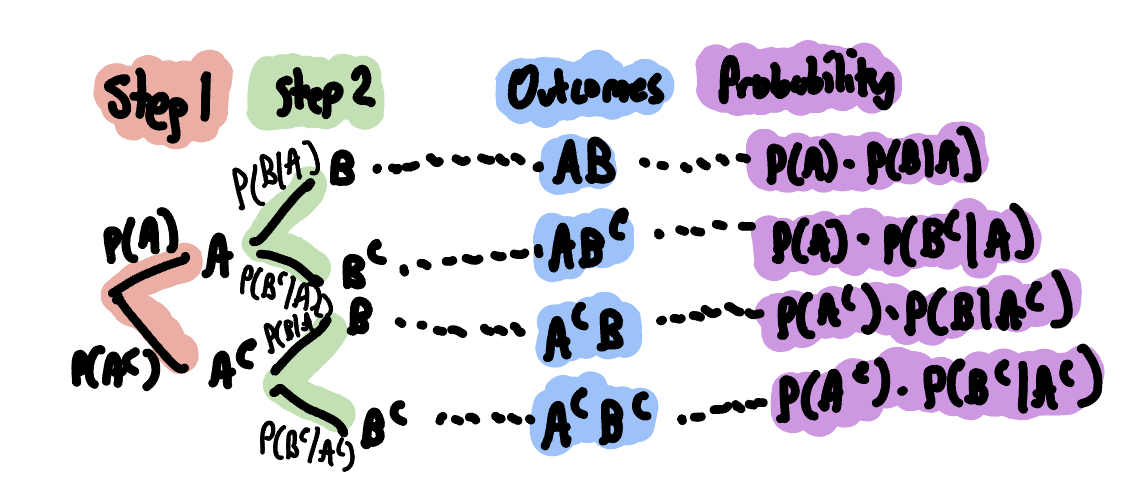
\includegraphics[width=0.5\textwidth]{tree.jpeg}
    \caption{Tree visualization for a generic two-step probability experiment}
    \label{fig:tree}
\end{figure}

$\hfill \break$
In this experiment, there are two starting outcomes, with two outcomes for each initial starting outcome. The above diagram explores visually how each outcome is related, and how the probability of each outcome can be calculated in the end. We can use a tree to visualize these outcomes, and further, visually see how we trace the probabilities through the tree, in order to help us compute the final probability for a given path.

\end{document}